\documentclass{beamer}

\usepackage[cm-default]{fontspec}
\usepackage{xunicode}
\usepackage{xltxtra}
\setmainfont[Mapping=tex-text]{DejaVu Sans}

\usepackage{graphicx}
\usepackage{amssymb}

\usetheme{Pittsburgh}
\useinnertheme{rounded}
\usefonttheme{serif}
\usecolortheme{beaver}

\title[Αναδρομικές Συναρτήσεις στο λ-λογισμό]{Αναπαράσταση Αναδρομικών Συναρτήσεων στο λ-λογισμό}
\author{Σταύρος Αρώνης, Ειρήνη Αρβανίτη}
\date{14 Σεπτεμβρίου 2010}
\institute{Εφαρμογές της λογικής στην Πληροφορική\\Σχολή ΗΜΜΥ, ΕΜΠ}

\AtBeginSection[]
{
  \begin{frame}<beamer>
    \frametitle{Επισκόπηση}
    \tableofcontents[currentsection, hideothersubsections]
  \end{frame}
}

\begin{document}

\begin{frame}
        \titlepage
        \begin{center}
                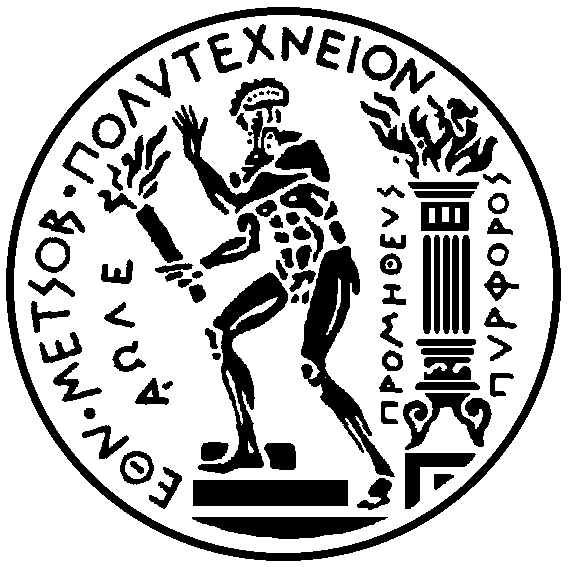
\includegraphics[height=2cm]{pyrforos.png}
        \end{center}
\end{frame}

\section*{Επισκόπηση}

\begin{frame}
  \tableofcontents[hidesubsections]
\end{frame}

\section{Πρωταρχικά αναδρομικές συναρτήσεις}

\subsection{Ορισμός}

\begin{frame}
        \frametitle{Ορισμός}
        \begin{itemize}
                \item   Οι \textbf{πρωταρχικά αναδρομικές συναρτήσεις} 
                                είναι συναρτήσεις με πεδίο ορισμού το \( \mathbb{N}^k \) 
                                και σύνολο τιμών το \( \mathbb{N} \).
                \pause
                \item   Η κλάση τους είναι η μικρότερη που περιέχει τις ακόλουθες
                                θεμελιώδεις συναρτήσεις και είναι κλειστή ως προς τα ακόλουθα
                                σχήματα κλεισίματος.
        \end{itemize}
\end{frame}

\subsection{Θεμελιώδεις συναρτήσεις}

\begin{frame}
        \frametitle{Θεμελιώδεις συναρτήσεις}
        \begin{itemize}
                \item Η σταθερή συνάρτηση με τιμή 0: \[Z_0=0\]
                \pause
                \item Η συνάρτηση που παίρνει έναν αριθμό και επιστρέφει τον επόμενο: \[S_1(n)=n+1\]
                \pause
                \item Οι συναρτήσεις προβολής: \[U^i_n(x_1,\ldots,x_i,\ldots,x_n)=x_i\]
        \end{itemize}
\end{frame}

\subsection{Σχήματα κλεισίματος}

\subsubsection{Σύνθεση}

\begin{frame}
        \frametitle{Σύνθεση}
        \begin{itemize}
                \item Αν έχουμε τις πρωταρχικά αναδρομικές συναρτήσεις: \[H_m, G1_n, \ldots, GM_n\]
                \pause
                \item Τότε και η \[F_n(x_1,\ldots,x_n) = H_m(G1_n(x_1,\ldots,x_n),\ldots,GM_n(x_1,\ldots,x_n))\]
                είναι πρωταρχικά αναδρομική.
        \end{itemize}
\end{frame}

\subsubsection{Πρωταρχική Αναδρομή}

\begin{frame}
        \frametitle{Πρωταρχική Αναδρομή}
        \begin{itemize}
                \item Αν έχουμε τις πρωταρχικά αναδρομικές συναρτήσεις: \[G_n, H_{n+2}\]
                \pause
                \item Τότε και η 
                \[
                        \left\{
                                \begin{array}{ll}
                                        F_n(x_1,\ldots,x_n, 0) &= G_n(x_1,\ldots,x_n) \\
                                        F_n(x_1,\ldots,x_n, S_1(y)) &= H_{n+2}(x_1,\ldots,x_n, y , F_n(x_1,\ldots,x_n, y))
                                \end{array}
                        \right.
                \]
                είναι πρωταρχικά αναδρομική.
        \end{itemize}
\end{frame}

\subsection{Παραδείγματα πρωταρχικά αναδρομικών συναρτήσεων}

\begin{frame}
        \frametitle{Παραδείγματα πρωταρχικά αναδρομικών συναρτήσεων}
        \begin{itemize}
                \item Η συνάρτηση προηγούμενος:
                \[
                        \left\{
                                \begin{array}{ll}
                                        P_1(0) &= Z_0\\
                                        P_1(S_1(x)) &= U^1_2(x,P(x))
                                \end{array}
                        \right.
                \]
                \pause
                \item Η συνάρτηση πρόσθεσης:
                \[
                        \left\{
                                \begin{array}{ll}
                                        Add_2(x, 0) &= U^1_1(x)\\
                                        Add_2(x, S_1(y)) &= S_1(U^3_3(x, y , Add_2(x, y)))
                                \end{array}
                        \right.
                \]
                \pause
                ή πιο απλά:
                \[
                        \left\{
                                \begin{array}{ll}
                                        Add_2(x, 0) &= x\\
                                        Add_2(x, S_1(y)) &= S_1(Add_2(x, y))
                                \end{array}
                        \right.
                \]
                \pause
                \item Η συνάρτηση αφαίρεσης:
                \[
                        \left\{
                                \begin{array}{ll}
                                        Sub_2(x, 0) &= x\\
                                        Sub_2(x, S_1(y)) &= P_1(Sub_2(x, y))
                                \end{array}
                        \right.
                \]
        \end{itemize}
\end{frame}

\begin{frame}
        \frametitle{Παραδείγματα πρωταρχικά αναδρομικών συναρτήσεων}
        \begin{itemize}
                \item Η συνάρτηση πολλαπλασιασμού:
                \[
                        \left\{
                                \begin{array}{ll}
                                        Mult_2(x, 0) &= Z_0\\
                                        Mult_2(x, S_1(y)) &= Add_2(x, Mult_2(x, y))
                                \end{array}
                        \right.
                \]
                \pause
                \item Η συνάρτηση << ίσο με 0 >>:
                \[
                        \left\{
                                \begin{array}{ll}
                                        EZ(0) &= S_1(Z_0)\\
                                        EZ(S_1(x)) &= Z_0
                                \end{array}
                        \right.
                \]
        \end{itemize}
\end{frame}

\subsection{Απαρίθμηση πρωταρχικά αναδρομικών συναρτήσεων}

\begin{frame}
        \frametitle{Απαρίθμηση πρωταρχικά αναδρομικών συναρτήσεων}
        \begin{itemize}
                \item Οι πρωταρχικά αναδρομικές συναρτήσεις είναι αριθμήσιμο σύνολο.
                \pause
                \item Για την απαρίθμηση μπορούμε να χρησιμοποιήσουμε π.χ. το 
                ακόλουθο σχήμα βασισμένο στα αριθμητικά του G\"odel
                \footnote{
                \htmladdnormallink{\tiny
                http://en.wikipedia.org/wiki/G\"odel\_number}
                {http://en.wikipedia.org/wiki/G\%C3\%B6del_number}}:
                \begin{itemize}
                        \item Οι θεμελιώδεις συναρτήσεις:
                        \[
                                \begin{array}{l}
                                        Z_0 \rightarrow 1 \\
                                        S_1 \rightarrow 2*3^1 \\
                                        U^i_n \rightarrow 2^2*3^n*5^i
                                \end{array}
                        \]
                \end{itemize}
        \end{itemize}
\end{frame}

\begin{frame}
        \frametitle{Απαρίθμηση πρωταρχικά αναδρομικών συναρτήσεων}
        \begin{itemize}
                \item Το σχήμα σύνθεσης:
                \begin{itemize}
                        \item Αν έχουμε την αντιστοίχιση:
                                \[\begin{array}{l}
                                        H_m \rightarrow N_H,\\
                                        G1_n \rightarrow N_{G1},\\
                                        \ldots,\\
                                        GM_n \rightarrow N_{GM}
                                \end{array}\]
                \pause
                        \item Τότε η \( F_n(x_1,\ldots,x_n) = H_m(G1_n(x_1,\ldots,x_n),\ldots,GM_n(x_1,\ldots,x_n)) \)
                        αντιστοιχεί στο:
                        \[
                                2^3*3^n*5^{N_H}*7^{N_{G1}}*\ldots*Prime_{m+3}^{N_{GM_n}}
                        \]
                \end{itemize}                   
        \end{itemize}
\end{frame}

\begin{frame}
        \frametitle{Απαρίθμηση πρωταρχικά αναδρομικών συναρτήσεων}
        \begin{itemize}
                \item Το σχήμα πρωταρχικής αναδρομής:
                \begin{itemize}
                        \item Αν έχουμε την αντιστοίχιση:
                                \[\begin{array}{l}
                                        G_n \rightarrow N_Γ,\\
                                        H_{n+2} \rightarrow N_H
                                \end{array}\]
                \pause
                        \item Τότε η 
                        \[\left\{
                                \begin{array}{ll}
                                        F_n(x_1,\ldots,x_n, 0) &= G_n(x_1,\ldots,x_n) \\
                                        F_n(x_1,\ldots,x_n, S_1(y)) &= H_{n+2}(x_1,\ldots,x_n, y , F_n(x_1,\ldots,x_n, y))
                                \end{array}
                        \right.\]
                        αντιστοιχεί στο:
                        \[
                                2^4*3^n*5^{N_G}*7^{H_H}
                        \]
                \end{itemize}                   
        \end{itemize}
\end{frame}

\begin{frame}
        \frametitle{Απαρίθμηση πρωταρχικά αναδρομικών συναρτήσεων}
        \begin{itemize}
                \item Η απαρίθμηση δεν αντιστοιχεί σε κάθε ακέραιο μια έγκυρη
                πρωταρχικά αναδρομική συνάρτηση αλλά είναι εφικτό να ελεγχθεί αν
                ένας ακέραιος αντιστοιχεί σε έγκυρη συνάρτηση:
                \pause
                \begin{itemize}
                        \item Παραγοντοποιούμε τον αριθμό
                \pause
                        \item Ελέγχουμε τη δύναμη του 2 για να δούμε αν είναι απλή περίπτωση
                \pause
                        \item Αν είναι σχήμα κλεισίματος, ελέγχουμε αναδρομικά κάθε μια συνάρτηση
                        που περιλαμβάνεται όπως και το ίδιο το σχήμα κλεισίματος.
                \end{itemize}
                \pause
                \item Είναι επίσης εύκολο να βρούμε πόσα ορίσματα εχει μια συνάρτηση που αντιστοιχεί σε έναν κωδικό
                \pause
                \item \(Legal(x)=0|1\) και \(Args(x)=n\)
        \end{itemize}
\end{frame}

\section{Αναδρομικές συναρτήσεις}

\subsection{Γιατί δεν αρκεί η πρωταρχική αναδρομή}

\begin{frame}
        \frametitle{Γιατί δεν αρκεί η πρωταρχική αναδρομή}
        \begin{itemize}
                \item Δεν είναι όλες οι << υπολογίσιμες >> συναρτήσεις
                πρωταρχικά αναδρομικές!
                \pause
                \item Έστω η συνάρτηση \(f(x)\) με τύπο:
                \[f(x)=\left\{
                        \begin{array}{ll}
                                0 &, Legal(x) \neq 1 \wedge Args(x) = 1\\
                                FX_1(x) + 1 &, otherwise
                        \end{array}
                \right.\]
                όπου \(FX_1\) η συνάρτηση με κωδικό \(x\).
                \pause
                \item Υπολογίσιμη συνάρτηση.
        \end{itemize}
\end{frame}

\begin{frame}
        \frametitle{Γιατί δεν αρκεί η πρωταρχική αναδρομή}
        \begin{itemize}
                \item Έστω ότι η \(f\) είναι πρωταρχικά αναδρομική.
                \pause
                \item Τότε έχει κάποιον κωδικό έστω \(N_f\).
                \pause
                \item Άρα \(f(N_f) = FN_f(N_f) + 1 = f(N_f) + 1\).
                \pause
                \item Άτοπο!
        \end{itemize}
\end{frame}

\begin{frame}
        \frametitle{Γιατί δεν αρκεί η πρωταρχική αναδρομή}
        \begin{itemize}
                \item Η συνάρτηση Ackermann:
                \[\left\{
                        \begin{array}{ll}
                                A(0,n) &= n+1\\
                                A(m,0) &= A(m-1,1)\\
                                A(m,n) &= A(m-1, A(m,n-1))
                        \end{array}
                \right.\]
                \pause
                \item Υπολογίσιμη.
                \pause
                \item Δεν μπορεί να γραφεί με πρωταρχική αναδρομή 
                \footnote{
                \htmladdnormallink{\tiny
                http://home.manhattan.edu/~gregory.taylor/thcomp/pdf-files/ackerman.pdf}
                {http://home.manhattan.edu/~gregory.taylor/thcomp/pdf-files/ackerman.pdf}}.
        \end{itemize}
\end{frame}

\subsection{Αναδρομικές συναρτήσεις}

\begin{frame}
        \frametitle{Αναδρομικές συναρτήσεις}
        \begin{itemize}
                \item Μερικές συναρτήσεις.
                \[F_n(a_1,\ldots,a_n)=\left\{
                        \begin{array}{l}
                                b\\
                                \bot
                        \end{array}
                \right.\]
                \pause 
                \item Περιλαμβάνουν:
                \begin{itemize}
                        \item Θεμελιώδεις συναρτήσεις.
                        \pause
                        \item Σχήματα κλεισίματος:
                        \begin{itemize}
                                \item Σύνθεση
                                \item Πρωταρχική αναδρομή
                                \pause
                                \item \textbf{Ελαχιστοποίηση}
                        \end{itemize}
                \end{itemize}
        \end{itemize}
\end{frame}

\subsection{Σχήμα ελαχιστοποίησης}

\begin{frame}
        \frametitle{Σχήμα ελαχιστοποίησης}
        \begin{itemize}
                \item Αν έχουμε την αναδρομική συνάρτηση \(F_{n+1}(y,x_1,\ldots,x_n)\)
                \pause
                \item Τότε και η:
                \[
                \small
                \begin{array}{ll}
                G_n =\\
                \mu y(x_1,\ldots,x_n) = z \Leftrightarrow 
                & \exists y_0,\ldots,y_n\:such\:that \\
                & y_i = F_{n+1}(i, x_1,\ldots, x_n),\:for\:i=0,1,\ldots,z \\
                & y_i > 0,\:for\:i=0,1,\ldots,z-1 \\
                & y_z = 0
                \end{array}
                \]
                είναι αναδρομική.
        \end{itemize}
\end{frame}

\subsection{Αοριστία}

\begin{frame}
        \frametitle{Αοριστία}
        \begin{itemize}
    	    \item Η χρήση του παραπάνω σχήματος εισάγει αοριστίες:
    	    \pause
            \item Αν \( y_i = F_{n+1}(i, x_1,\ldots, x_n) \) δεν είναι ποτέ ίσο με \( 0 \).
            \pause
            \item Αν \( y_i > 0,\:for\:i=0,1,\ldots,w-1 \) και \( y_w \) δεν ορίζεται.
        \end{itemize}
\end{frame}

\subsection{Παραδείγματα αναδρομικών συναρτήσεων}

\begin{frame}
        \frametitle{Παραδείγματα αναδρομικών συναρτήσεων}
        \begin{itemize}
                \item Αναπαράσταση της συνάρτησης Ackermann με αναδρομή
        \end{itemize}
\end{frame}

\section{Στοιχεία λ-λογισμού}

\subsection{Συντακτικό}

\begin{frame}
        \frametitle{Συντακτικό}
        \begin{itemize}
                \item Ένας λ-όρος μπορεί να είναι μια μεταβλητή.\[x\]
                \pause
                \item Αν \(t\) είναι λ-όρος και \(x\) είναι μεταβλητή, τότε \[\lambda x . t\]
                είναι επίσης λ-όρος.
                \pause
                \item Αν \(t, u\) είναι λ-όροι, τότε \[(t)u\]
                είναι επίσης λ-όρος.
        \end{itemize}
\end{frame}

\subsection{Αντικατάσταση}

\begin{frame}
        \frametitle{Αντικατάσταση}
        \begin{itemize}
        	\item Αν \(t\), \(M\) είναι λ-όροι και \(x\) είναι μεταβλητή, τότε η αντικατάσταση της \(x\)
            από τον \(t\) στον όρο \(M\), συμβολίζεται με \(M[x:=t]\) \\
            \pause
            \item \[x[x:=t] \equiv t\]
            \pause
            \item \[y[x:=t] \equiv y\]
                                    
        \end{itemize}
\end{frame}

\begin{frame}
        \frametitle{Αντικατάσταση}
        \begin{itemize}
        	
            \item \[(PQ)[x:=t] \equiv (P[x:=t])(Q[x:=t])\]
            \pause
            \item \[(\lambda y . P)[x:=t] \equiv \lambda y . (P[x:=t])\]
            \pause
            \item \[(\lambda x . P)[x:=t] \equiv \lambda x . P\]
            
        \end{itemize}
\end{frame}

\subsection{β-συστολή}

\begin{frame}
        \frametitle{β-συστολή}
        \begin{itemize}
        	
            \item $\rightarrow _\beta$ είναι η μικρότερη διμελής σχέση στο $\Lambda$ ώστε να ισχύει ότι 
                  \[(\lambda x . P)Q \rightarrow _\beta P[x:=Q]\]
            \pause
                  και η οποία είναι κλειστή για τους ακόλουθους κανόνες:
            \pause
            \item \[P \rightarrow _\beta P^{\prime}  \Rightarrow \forall x \in V : \lambda x . P \rightarrow _\beta \lambda x .    P^{\prime}\]
            \pause
            \item \[P \rightarrow _\beta P^{\prime}  \Rightarrow \forall Z \in \Lambda : P Z \rightarrow _\beta P^{\prime} Z\]
			\pause
            \item \[P \rightarrow _\beta P^{\prime}  \Rightarrow \forall Z \in \Lambda : Z P \rightarrow _\beta Z P^{\prime}\]
            
        \end{itemize}
\end{frame}

\begin{frame}
        \frametitle{β-συστολή}
        \begin{itemize}
        	
            \item $(\lambda x . P)Q$: $\beta$ - \textit{redex}
            \pause
			\item $P[x:=Q]$: $\beta$ - \textit{contractum}
            \pause
            \item ´Ενας όρος \(M\) είναι μία \textit{$\beta$ - κανονική μορφή} εάν δεν υπάρχει όρος \(N\) ώστε $M \rightarrow _\beta N$.
            
        \end{itemize}
\end{frame}

\subsection{β-αναγωγή}

\begin{frame}
        \frametitle{β-αναγωγή}
        \begin{itemize}
        	
            \item Η σχέση $\twoheadrightarrow _\beta$ είναι η μεταβατική και αυτοπαθής κλειστότητα της σχέσης
                  $\rightarrow _\beta$ \\ Συνεπώς είναι κλειστή για τους κανόνες: 
            \pause
            \item \[P \rightarrow  _{\beta} P ^{\prime} \Rightarrow P \twoheadrightarrow _{\beta} P ^{\prime}\]
            \pause
            \item \[P \twoheadrightarrow _{\beta} P ^{\prime} \cap P ^{\prime} \twoheadrightarrow _{\beta} P ^{\prime \prime}
                  \Rightarrow P \rightarrow ^{\star} _{\beta} P ^{\prime \prime}\]
			\pause
            \item \[P \twoheadrightarrow _{\beta} P\]
            
        \end{itemize}
\end{frame}

\begin{frame}
        \frametitle{β-συστολή}
        \begin{itemize}
        \item Ισχύει η ακόλουθη πρόταση:\\
        		\[
                \small
                \begin{array}{ll}
                M \twoheadrightarrow _\beta N \Leftrightarrow 
                & $Είτε $ M \equiv N $ είτε υπάρχουν $ M_1, M_2,\ldots M_n $ ώστε $ \\
                & M \equiv M_1 $ και N $ \equiv M_n $ και για κάθε $ i (1 \leq i \leq n-1),\\
                & M_i \twoheadrightarrow _\beta M_{i+1}
                \end{array}
                \]
		\end{itemize}
\end{frame}

\subsection{β-ισοδυναμία}

\begin{frame}
        \frametitle{β-ισοδυναμία}
        \begin{itemize}
        	
            \item Η σχέση $ =_\beta$ είναι η μεταβατική, αυτοπαθής και συμμετρική κλειστότητα της σχέσης
                  $\rightarrow _\beta$ \\ Συνεπώς είναι κλειστή για τους κανόνες: 
            \pause
            \item \[P \rightarrow  _\beta P^\prime \Rightarrow P  =_\beta P^\prime \]
            \pause
            \item \[P  =_\beta P^\prime \cap P^\prime =_\beta P ^{\prime \prime}
                  \Rightarrow P =_\beta P ^{\prime \prime}\]
			\pause
            \item \[P =_\beta P\]
            \pause
            \item \[P  =_\beta P^\prime \Rightarrow P^\prime =_\beta P\]
            
        \end{itemize}
\end{frame}

\begin{frame}
        \frametitle{β-ισοδυναμία}
        \begin{itemize}
        		\item Ισχύει η ακόλουθη πρόταση:\\
        		\[
                \small
                \begin{array}{ll}
                M =_\beta N \Leftrightarrow 
                & $ Υπάρχουν $ M_1, M_2,\ldots M_n $ με $ M \equiv M_1 $ και $ N \equiv M_n \\
                & $ και για κάθε i $ (1 \leq i \leq n-1) $ έχουν $ M_i \twoheadrightarrow _\beta M_{i+1}\\
                & $ ή $ M_{i+1} \twoheadrightarrow _\beta M_i
                \end{array}
                \] \pause
                \item \textbf{Πόρισμα}: Ο $\lambda$-λογισμός ως θεωρία της $\beta$-ισότητας είναι συνεπής θεωρία.					\pause
				\item \textbf{Απόδειξη}: $\lambda x . x \neq _\beta \lambda x . \lambda y . x$
		\end{itemize}
\end{frame}

\subsection{Κανονικοποίηση}

\begin{frame}
\frametitle{Κανονικοποίηση}
\begin{itemize}
\item \textbf{Θεώρημα Church-Rosser:} Αν  $t \twoheadrightarrow _\beta u, v$  τότε μπορεί να βρεθεί $w$ τέτοιο ώστε $ u, v \twoheadrightarrow _\beta w$.\pause

\begin{figure}
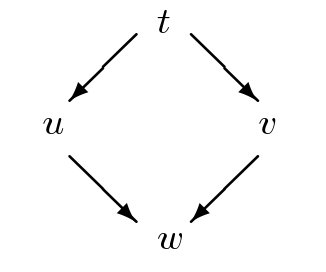
\includegraphics[scale=0.3]{CR.jpg} 
\end{figure}\pause
\item \textbf{Ορισμός}: Έστω $t \twoheadrightarrow _\beta u$ και $u$ είναι $\beta$-κανονική μορφή. Τότε ο όρος $u$ λέγεται $\beta$-κανονική μορφή του $t$.\pause
\item \textbf{Πόρισμα}: Ένας όρος $t$ έχει το πολύ μια κανονική μορφή. 
\end{itemize}
\end{frame}

\begin{frame}
\frametitle{Κανονικοποίηση}
\begin{itemize}
\item \textbf{Πόρισμα}:  $u =_\beta v \Leftrightarrow$ Υπάρχει όρος $t$ ώστε $u, v \twoheadrightarrow _\beta t$.\pause
\item $(\Leftarrow)$ Προφανές από τον ορισμό της $\beta$-ισοδυναμίας.\pause
\item $(\Rightarrow)$ Aν  κάποιος μπορεί να συμπεράνει ότι $u = v$, τότε είναι εύκολο να παρατηρήσει ότι υπάρχουν όροι $u = t_0, t_1,\ldots, t_{2n-1}, t_{2n} = v$. Εφαρμόζοντας επανειλημμένα το θεώρημα Church-Rosser, καταλήγουμε σε έναν όρο	$w$ τέτοιον ώστε $u, v \leadsto w$.\pause
\begin{figure} [!ht]
\centering
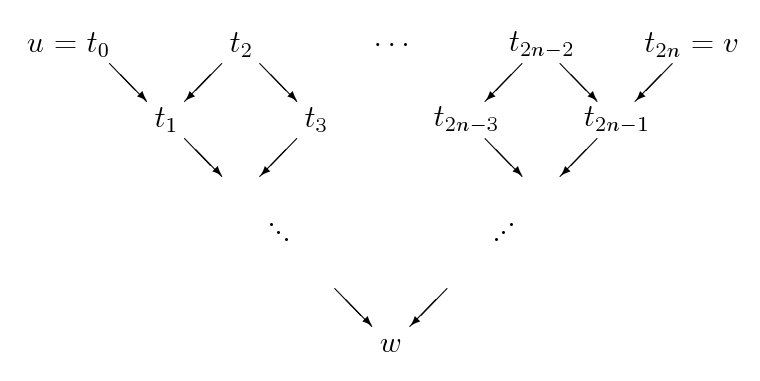
\includegraphics[scale=0.3] {CR1.jpg}
\end{figure}
\end{itemize}
\end{frame}

\begin{frame}
\frametitle{Κανονικοποίηση}
\begin{itemize}
\item Δεν έχουν όλοι οι όροι κανονικές μορφές, π.χ. ο όρος $\Omega \equiv  (\lambda x . xx) \lambda x . xx$. Αν όμως υπάρχει, τότε είναι μοναδική. \pause
\item Ένας όρος ο οποίος έχει κανονική μορφή ονομάζεται κανονικοποιήσιμος. Αυτό δε συνεπάγεται ότι οποιαδήποτε αναγωγή οδηγεί στην κανονική μορφή του. \pause
\item Κάθε όρος που έχει άπειρη αναγωγή περιέχει τον όρο $\Omega$. Ωστόσο, το αντίστροφο δεν ισχύει.\pause
\item Ένας όρος που δεν έχει καμία άπειρη αναγωγή ονομάζεται ισχυρά κανονικοποιήσιμος. 
\end{itemize}
\end{frame}

\begin{frame}
\frametitle{Αριστερότερη Αναγωγή}
\begin{itemize}
\item \textbf{Αριστερότερο redex} ενός μη κανονικού όρου $t$ είναι το redex στο οποίο το "$(\lambda$" βρίσκεται αριστερότερα από κάθε άλλο "$(\lambda$" του $t$. \pause
\item \textbf{Αριστερότερη αναγωγή} καλείται μία ακολουθία $t_0, t_1, \ldots, t_n, \ldots$ τέτοια ώστε $\forall n: t_n \rightarrow _\beta t_{n+1}$ με συστολή του αριστερότερου redex στον $t_n$. \pause
\item \textbf{Συμβολισμός:} $t \rightarrow _l t^\prime$ , $t \twoheadrightarrow _l t^\prime$ \pause
\item Για δεδομένα $t$, $n$ η αριστερότερη αναγωγή είναι μοναδική. Αν $t$ κανονικοποιήσιμος τότε η αριστερότερη αναγωγή καταλήγει στην κανονική μορφή του $t$. \pause
\end{itemize}
\end{frame}

\begin{frame}
\frametitle{Αναγωγή κεφαλής}
\begin{itemize}
\item \textbf{Πρόταση:} Κάθε $\lambda$-όρος $t$ γράφεται μοναδικά με μία από τις ακόλουθες μορφές: \pause
 \[(1): \lambda x_1 \ldots \lambda x_n . (x) t_1 \ldots t_m\] 
 \[(2): \lambda x_1 \ldots \lambda x_n . ((\lambda x . u) v) t_1 \ldots t_m\] \pause
\item \textbf{Απόδειξη:} Με επαγωγή στον όρο $t$. \pause
\item $t$ μεταβλητή: (1) όπου $n=m=0$ \pause
\item $t = \lambda x . t^\prime$: Από Ε.Υ. $t^\prime$ γράφεται κατάλληλα, συνεπώς το ίδιο και ο $t$ \pause
\item $t = (t^\prime) t^{\prime \prime}$:
	\begin{itemize}
	\item $t^\prime$ $\lambda$-αφαίρεση: (2) όπου $n=m=0$ \pause
	\item αν $t^\prime$ δεν είναι $\lambda$-αφαίρεση, τότε $t^\prime = (w) w_1 \ldots w_k$, όπου $w$ μεταβλητή ή redex, άρα  $t = ((w) w_1 \ldots w_k) t^{\prime \prime}$, δηλαδή (1) ή (2) όπου $n=0$
	\end{itemize}
\end{itemize}
\end{frame}

\begin{frame}
\frametitle{Αναγωγή κεφαλής}
\begin{itemize}
\item Κάθε όρος $t = \lambda x_1 \ldots \lambda x_n . (x) t_1 \ldots t_m$ ονομάζεται κανονική μορφή κεφαλής.\pause
\item Επιπλέον, αν $t = \lambda x_1 \ldots \lambda x_n . ((\lambda x . u) v) t_1 \ldots t_m$, τότε $(\lambda x . u) v$ ονομάζεται redex κεφαλής.\pause
\item Το redex κεφαλής (αν υπάρχει) είναι το αριστερότερο redex, ενώ το αντίστροφο δεν ισχύει.\pause
\item Για δεδομένο όρο $t$ η αναγωγή κεφαλής είναι μοναδική.
\item \textbf{Συμβολισμός:} $t \rightarrow _h t^\prime$ , $t \twoheadrightarrow _h t^\prime$ \pause
\end{itemize}
\end{frame}

\begin{frame}
\frametitle{Επιλυσιμότητα}
\begin{itemize}
\item Ο κλειστός όρος $t$ είναι επιλύσιμος αν υπάρχουν $v_1, \ldots, v_n, (n \geqslant 0)$ ώστε
 $ (t) v_1 \ldots v_n =_\beta \mathbb{I} $ \pause
 \item Τυχών όρος $t$ είναι επιλύσιμος αν η κλειστότητα $\lambda \overrightarrow{x} . t$ είναι επιλύσιμος. \pause
 \item \textbf{Πρόταση:} $(t) v$ επιλύσιμος $ \Rightarrow t$ επιλύσιμος. \pause
 \item Επιπλέον, για κάθε λ-όρο $t$ τα ακόλουθα είναι ισοδύναμα:
 	\begin{enumerate}
 	\item $t$ επιλύσιμος
 	\item $t =_\beta$ κανονική μορφή κεφαλής
 	\item η αναγωγή κεφαλής του $t$ τερματίζει 	
 	\end{enumerate}
\end{itemize}
\end{frame}

\section{Αναπαράσταση αναδρομικών συναρτήσεων}

\subsection{Church Numerals}

\begin{frame}
        \frametitle{Church Numerals}
        \begin{itemize}
                \item Αναπαράσταση του \( \mathbb{N} \) στο λ-λογισμό:
                \pause
	        	\[ \begin{array}{l}
	        		0 \rightarrow \lambda f . \lambda x . x \\
	        		1 \rightarrow \lambda f . \lambda x . (f) x \\
	        		2 \rightarrow \lambda f . \lambda x . (f) (f) x \\
	        		\ldots \\
	        		n \rightarrow \lambda f . \lambda x . \underbrace{(f) \ldots (f)}_n x \\
	        		\ldots
	        	\end{array} \]
	        	\pause
                \item Αν \(n \) είναι Church Numeral και \(t, u\) είναι λ-όροι, τότε
                \[ n\:t\:u =_\beta (t)^n u \]
        \end{itemize}
\end{frame}

\subsection{Θεμελιώδεις συναρτήσεις}
\begin{frame}
        \frametitle{Αναπαράσταση μερικών συναρτήσεων}
        \begin{itemize}
                \item Έστω $\phi : \mathbb{N}^n \rightarrow \mathbb{N}$ μερική συνάρτηση και $\Phi \belongs $
                \pause
               
        \end{itemize}
\end{frame}




\begin{frame}
        \frametitle{Θεμελιώδεις συναρτήσεις}
        \begin{itemize}
                \item Η σταθερή συνάρτηση με τιμή 0: \[Z_0=\lambda f . \lambda x . x\]
                \pause
                \item Η συνάρτηση που παίρνει έναν αριθμό και επιστρέφει τον επόμενο: \[S_1(n)=\lambda n . \lambda f . \lambda x . (f) (n) f x\]
                \pause
                \item Οι συναρτήσεις προβολής: \[U^i_n(x_1,\ldots,x_i,\ldots,x_n)= \lambda x_1 . \ldots \lambda x_i . \ldots \lambda x_n . x_i\]
        \end{itemize}
\end{frame}
\subsection{Σχήματα κλεισίματος}
\subsubsection{Σύνθεση}
\begin{frame}
        \frametitle{Σύνθεση}
        \begin{itemize}
                \item Απλή ιδέα: \[o = \lambda f. \lambda g. \lambda x . (f) (g) x\]
                \pause
                \item Τότε αν $n \geqslant 1$ είναι Church Numeral και $S, h$ κλειστοί $\lambda$-όροι, τότε
                \[ ((n) \lambda g . g o S) h \twoheadrightarrow _h (\lambda g . g o S)^n h
                   \twoheadrightarrow _h \lambda x . (h) (S)^n x \] \pause
                 \item Απόδειξη: Επαγωγή στο $n$.
        \end{itemize}
\end{frame}

\begin{frame}
        \frametitle{Σύνθεση}
        \begin{itemize}
                \item Έστω $\Phi, w$ δύο $\lambda$-όροι, $m$ Church Numeral. Όρίζουμε $<\Phi, w> = ((w) \lambda g . g o S_1) \Phi \Omega$. Τότε:
                \pause
                \item αν $w$ μη επιλύσιμος, τότε $<\Phi, w>$ μη επιλύσιμος. \pause
                \item αν $w =_\beta m$ τότε $<\Phi, w> =_\beta \Phi m$ \pause
                \item Απόδειξη: 
                \[
                \small
                \begin{array}{ll}
                w =_\beta m \Rightarrow <\Phi, w>
                & =_\beta ((m) \lambda g . g o S_1) \Phi \Omega \\
                & =_\beta (\lambda g . g o S_1)^m \Phi \Omega \\
                & =_\beta (\lambda x . (\Phi) (S_1)^m x) \Omega \\
                & =_\beta (\Phi) (S_1)^m \Omega \\
                & =_\beta \Phi m
                \end{array}
                \]           	
           
        \end{itemize}
\end{frame}

\begin{frame}
        \frametitle{Σύνθεση}
        \begin{itemize}
                \item ´Εστω $<\Phi, w_1,\ldots, w_k> := <<\Phi, w_1,\ldots, w_{k-1}>, w_k>$. \\
                  Αν $\Phi, w_1,\ldots, w_k$ είναι λ-όροι τ.ω. κάθε $w_i$ είναι β-ισοδύναμο με φυσικό του Church ή μη επιλύσιμο, τότε: \pause
                 \item αν ένα από τα $w_i$ είναι μη επιλύσιμο, τότε και $<\Phi, w_1,\ldots, w_k>$ μη επιλύσιμος. \pause
                 \item αν $\forall i: w_i =_\beta n_i$, τότε $<\Phi, w_1,\ldots, w_k> =_\beta \Phi n_1 \ldots n_k$   
        \end{itemize}
\end{frame}

\begin{frame}
        \frametitle{Σύνθεση}
        \begin{itemize}
                \item \textbf{Πρόταση:} Αν $f_1,\ldots,f_k : \mathbb{N}^n \rightarrow \mathbb{N}, g : \mathbb{N}^k \rightarrow \mathbb{N}$ είναι ισχυρά αναπαραστάσιμες στο λ-λογισμό, τότε και η σύνθεση 
                 $g(f_1,\ldots,f_k)$ είναι ισχυρά αναπαραστάσιμη. \pause
                 \item \textbf{Απόδειξη:} Αν $\Phi_1, \ldots, \Phi_k, \Psi$ αναπαριστούν ισχυρά τις
                  $f_1,\ldots, f_k, g$, τότε
                  \[X = \lambda x_1 \ldots \lambda x_n . <\Psi, \Phi_1 x_1 \ldots x_n, \ldots, \Phi_k x_1 \ldots x_n> \]
                  αναπαριστά ισχυρά τη σύνθεση $g(f_1,\ldots,f_k)$. 
        \end{itemize}
\end{frame}

\subsubsection{Πρωταρχική Αναδρομή}
\subsection{Σχήμα ελαχιστοποίησης}
\end{document}
